\chapter{Пряма на площині}

\section{Різні способи задання ліній на площині}

Одним із найважливіших завдань аналітичної геометрії є представлення лінії
на площині за допомогою рівняння, що зв’язує координати кожної точки цієї лінії.
Нехай маємо на площині $P$ декартову прямокутну систему координат та деяку
лінію $L$.

\begin{definition}
	\textbf{Рівняння лінії $L$} --- це рівняння $F(x,y) = 0$, якому задовольняють
	координати $x$ та $y$ кожної точки цієї лінії. 
\end{definition}

Інакше кажучи, лінія – це геометричне місце точок, координати яких
задовольняють рівняння. Лінію $L$ можна задавати таким чином. 

1) \textbf{Неявний спосіб:} $F(x,y) = 0$. Функція $y$ від $x$ (чи $x$ від $y$) задана неявно.
Приклад: $x^2 + y^2 = R^2$ --- рівняння кола радіуса R з центром у початку координат.

2) \textbf{Явний спосіб:} $y = f(x)$. Функція $y$ від $x$ задана явно. Для побудови графіка
цієї функції складається таблиця значень $x$ та $f(x)$, ці пари точок позначаються на
площині та з’єднуються плавною лінією.
Приклад: $y = \pm\sqrt{R^2 - x^2}$. 

3) \textbf{Параметричне представлення:} $\left\{\begin{array}{l}
	x = x(t) \\
	y = y(t) \\	
\end{array}\right., t \in D$.
	
Щоб побудувати графік
такої функції треба скласти таблицю для $x(t)$ і $y(t)$ для однакових значень
параметра $t$ , що пробігає числову множину $D$ . Виключення з двох рівнянь
параметра $t$ приводить до неявного способу задання даної лінії $L$. 
Приклад: $\left\{\begin{array}{l}
	x = R\cos t \\
	y = R\sin t \\	
\end{array}\right., t \in [0, 2\pi]$.

\subsection*{Приклади графіків параметричних функцій:}

Приклад 1: циклоїда $\left\{\begin{array}{l}
	x = a(t - \sin t) \\
	y = a(1 - \cos t) \\	
\end{array}\right., t \in [-\infty, +\infty], a>0$.

Таку лінію описує фіксована точка кола радіуса a, що котиться по всій осі $Ox$.
Очевидно, що $y \in [0, 2a]$, а $y = 0$ при $1 - \cos t = 0\Rightarrow \cos t = 1 \Rightarrow t = 0, \pm2\pi, \pm4\pi$.

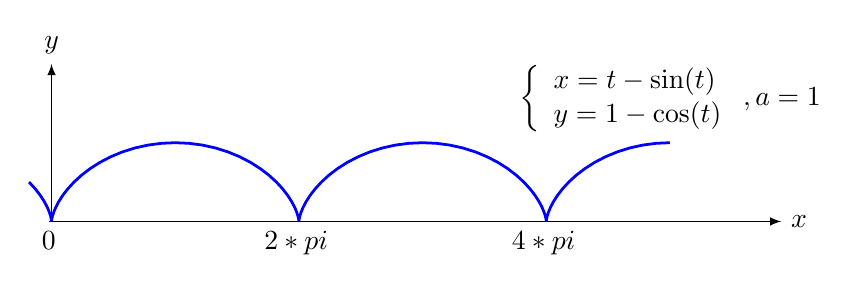
\begin{tikzpicture}[scale=.5]
  	\coordinate (O) at (0,0);
  	\coordinate (A) at (0,4);
  	\def\r{1} % radius
  	\def\c{1.4} % center
  	\coordinate (C) at (\c, \r);
  	
  	\draw[-latex] (O) -- (A) node[anchor=south] {$y$};
  	\draw[-latex] (O) -- (5.9*pi,0) node[anchor=west] {$x$};
	\foreach \pos in {0, 2*pi, 4*pi}
  		\draw[shift={(\pos,0)}] (2pt,0pt) -- (-2pt,0pt) node[below] {$\pos$};
  	\draw[blue,domain=-0.5*pi:5*pi,samples=100, line width=1] 
       	plot ({\x - sin(\x r)},{1 - cos(\x r)}) node[anchor=south, black]{$\left\{\begin{array}{l}
			x = t - \sin(t) \\
			y = 1 - \cos(t) \\	
		\end{array}\right., a=1$};
\end{tikzpicture}

Приклад 2: астроїда $\left\{\begin{array}{l}
	x = a\cos^3 t \\
	y = a\sin^3 t \\	
\end{array}\right., t \in [0, 2\pi]$.

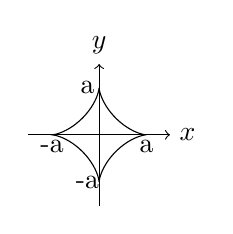
\begin{tikzpicture}[scale=0.6]
	\draw[->] (-1.5,0) -- (1.5,0) node[right] {$x$};
	\draw[->] (0,-1.5) -- (0,1.5) node[above] {$y$};    
    
   	\draw[domain=0:2*pi, samples=100] plot ({(cos(deg(\x)))^3},{(sin(deg(\x)))^3});
   	\draw (1,-0.25) node{a};
    \draw (-0.25,1) node{a};
    \draw (-1,-0.25) node{-a};
    \draw (-0.25,-1) node{-a};
\end{tikzpicture}
\parbox[b]{9cm}{Запишемо рівняння астроїди в неявному вигляді:

$\left(\dfrac{x}{a}\right)^{2/3} + \left(\dfrac{y}{a}\right)^{2/3}
= \cos^2 t + \sin^2 t = 1$

$\Rightarrow x^{2/3} + y^{2/3} = a^{2/3}$.}
	
4) Представлення лінії у полярній системі координат. На площині задана
полярна система координат, якщо задано:
\begin{enumerate}
	\item точка $O$ полюс;
	\item полярна вісь $\rho$ промінь, що виходить з точки $O$.	
\end{enumerate}	


	\begin{wrapfigure}{l}{100px}
		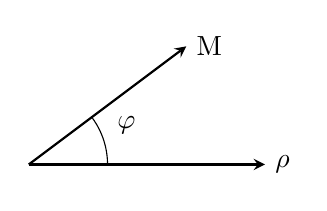
\begin{tikzpicture}[scale=0.5]
			\draw[-stealth, thick] (0,0) -- (6,0) node[anchor=west]{$\rho$};
			\draw[-stealth, thick] (0,0) -- (4,3) node[anchor=west]{M};
				
			\draw[black] (2,0) arc (0:36:2);
			\draw (2,1) node[anchor=west]{$\varphi$};
		\end{tikzpicture}
	\end{wrapfigure}

Тоді положення будь-якої точки $M$ на площині
визначається парою чисел $(\rho, \varphi)$, де полярний радіус
$\rho \geqslant 0$ --- довжина вектора $\overline{OM}$, а полярний кут $\varphi$ це
кут між віссю $\rho$ і $\overline{OM}$, який відраховується проти
годинникової стрілки. Якщо точка $M$ має декартові координати $(x, y)$ і цій парі
чисел відповідає пара $(\rho, \varphi)$, то ця відповідність буде взаємно однозначною, якщо
$\varphi \in [0, 2\pi]$ або $\varphi \in [-\pi, \pi]$. Легко вивести наступні співвідношення (перехід від
полярної системи координат до декартової, і навпаки):

\begin{equation}\label{fromPolarToDekart}
	\left\{\begin{array}{l}
		x = \rho \cos \varphi \\
		y = \rho \sin \varphi \\
	\end{array}\right.
\end{equation}

\begin{equation}\label{fromDekartToPolar}
	\left\{\begin{array}{l}
		\rho = \sqrt{x^2 + y^2} \\
		\left\{\begin{array}{l}
			\cos \varphi = \dfrac{x}{\sqrt{x^2 + y^2}} \\
			\sin \varphi = \dfrac{y}{\sqrt{x^2 + y^2}} \\
		\end{array}\right. \\
	\end{array}\right.
\end{equation}

Приклад: Лемніската Бернуллі $(x^2 + y^2)^2 = a^2(x^2 - y^2), a > 0$.

\parbox{140px}{\begin{tikzpicture}[scale=0.5]
  	\begin{polaraxis}[style=black!10, ticklabel style=black, xticklabel=$\pgfmathprintnumber{\tick}^\circ$]
    	\addplot [thick, black, domain=0:45, samples=50] {2*sqrt(cos(2*x))};
   	 	\addplot [thick, black, domain=-45:0, samples=50] {2*sqrt(cos(2*x))};
   	 	\addplot [thick, black, domain=135:225, samples=100] {2*sqrt(cos(2*x))};
    \end{polaraxis}
\end{tikzpicture}}
\parbox{7.2cm}{З формул \ref{fromDekartToPolar} випливає, що
	$\rho^4 = a^2\rho^2(\cos^2 \varphi - \sin^2 \varphi)$, тобто
	$\rho^2 = a\cos 2 \varphi$ або $\rho = \sqrt{a\cos 2 \varphi}$.
	Область визначення: $\cos 2\varphi \geqslant0$,
	тобто $\varphi \in \left[-\dfrac{\pi}{4}, \dfrac{\pi}{4}\right] \cup \left[\dfrac{3\pi}{4}, \dfrac{5\pi}{4}\right]$.
}

\section{Пряма на площині}

Нехай дано пряму $L$.

\begin{definition}
	\textbf{Нормальний вектор прямої $L$} --- це довільний ненульовий вектор $\overline{n}$, перпендикулярний прямій $L$.
\end{definition}

\noindent\parbox{2.8cm}{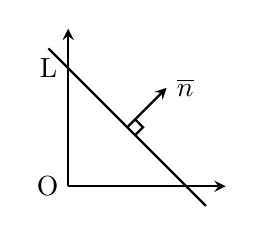
\begin{tikzpicture}[scale=0.5]
	\draw(0,0) node[anchor=east]{O};
  	\draw[-stealth, thick] (0,0) -- (4,0);
	\draw[-stealth, thick] (0,0) -- (0,4);
	\draw[thick] (3.5,-0.5) -- (-0.5,3.5)  node[anchor=north]{L};
	\draw[-stealth, thick] (1.5,1.5) -- (2.5,2.5) node[anchor=west]{$\overline{n}$};
	\draw[thick] (1.7,1.7) -- (1.9,1.5) -- (1.7,1.3);
\end{tikzpicture}}
\parbox{\textwidth - 2.9cm}{
	$\overline{n} \perp L; \overline{n} \neq \overline{0}$ --- нормальний вектор прямої.
	Зауважимо, що нормальних векторів існує безліч --- з точністю до ненульової константи.
}

Нехай задано точку $M_0(x_0, y_0)$. Складемо рівняння прямої, що проходить
через точку $M_0(x_0, y_0)$ перпендикулярно до вектора $\overline{n}(A, B)$.

Для довільної точки $M(x, y)$ шуканої прямої вектор $\overline{M_0 M} = (x-x_0, y-y_0)$ є
перпендикулярним вектору $\overline{n}$: $\overline{M_0 M} \perp \overline{n}$, тобто $(\overline{M_0 M}, \overline{n}) = 0$. Отримали:
$A(x-x_0) + B(y-y_0) = 0$ --- рівняння прямої через точку $M_0(x_0, y_0)$ та нормальний вектор $\overline{n}(A, B)$.

Побудуємо загальне рівняння прямої. Розкривши дужки, маємо $Ax + By - (Ax_0 + By_0) = 0$, де $A$ і $B \neq 0$
одночасно. Позначивши $C = -(Ax_0 + By_0)$, отримуємо 

\begin{center}
	$Ax + By + C = 0$ --- \textbf{загальний вигляд прямої}.
\end{center}

\section{Неповні рівняння прямої}

\begin{definition}
	Загальне рівняння $Ax + By + C = 0$ --- це \textbf{повне рівняння прямої}, якщо всі його
	коефіцієнти $A \neq 0, B \neq 0, C \neq 0$ (тобто $ABC \neq 0$). Якщо ж хоча б один коефіцієнт
	дорівнює нулю, то це \textbf{неповне рівняння прямої}.
\end{definition}

Розглянемо можливі випадки неповних рівнянь.
\begin{enumerate}
\item $C = 0; L: Ax + By = 0$ --- пряма $L$ проходить через точку $O(0,0)$.
\item $B = 0; L: Ax + C = 0;$ $\overline{n}(A, 0) \perp Oy, L \parallel Oy$.
\item $A = 0; L: By + C = 0;$ $\overline{n}(0, B) \perp Ox, L \parallel Ox$.
\item $B = 0, C = 0; L: Ax = 0$ --- пряма $L$ співпадає з віссю $Oy$.
\item $A = 0, C = 0; L: By = 0$ --- пряма $L$ співпадає з віссю $Ox$.
\end{enumerate}

\section{Рівняння прямої у відрізках}

Розглянемо повне рівняння прямої $L: Ax + By + C = 0$, де $ABC \neq 0$.

\begin{center}
	\parbox{4cm}{
		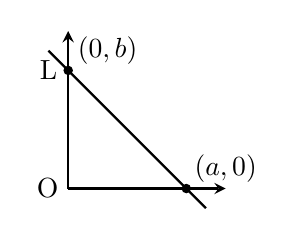
\begin{tikzpicture}[scale=0.5]
			\draw(0,0) node[anchor=east]{O};
			\draw[-stealth, thick] (0,0) -- (4,0);
			\draw[-stealth, thick] (0,0) -- (0,4);
			\draw[thick] (3.5,-0.5) -- (-0.5,3.5)  node[anchor=north]{L};
			\draw (1,3.5) node{$(0,b)$};
			\draw (4,0.5) node{$(a,0)$};
			\filldraw[black] (3,0) circle (3pt);
			\filldraw[black] (0,3) circle (3pt);		
		\end{tikzpicture}
	}
	\parbox{4cm}{
		$$Ax + By = -C;$$
		
		$$\dfrac{x}{-\dfrac{C}{A}} + \dfrac{y}{-\dfrac{C}{B}} = 1.$$
	}
\end{center}

Позначимо $a = -\dfrac{C}{A}, b = -\dfrac{C}{B}$. Тоді маємо рівняння прямої “у відрізках”:

$$\dfrac{x}{a} + \dfrac{y}{b} = 1$$

Геометричний зміст чисел $a$ і $b$: вони дорівнюють величинам відрізків, які
відсікає пряма $L$ на осях $Ox$ та $Oy$ відповідно.

\section{Канонічне рівняння}

\begin{definition}
	\textbf{Напрямний вектор} прямої $L$ --- це довільний ненульовий вектор $q \neq \overline{0}$, що паралельний прямій $L$.
\end{definition}

\parbox{100px}{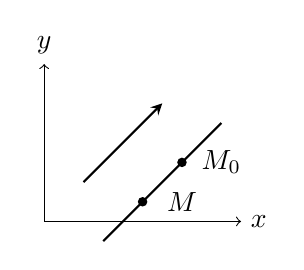
\begin{tikzpicture}[scale=0.5]
	\draw[->] (0,0) -- (5,0) node[right] {$x$};
	\draw[->] (0,0) -- (0,4) node[above] {$y$}; 

	\draw[-stealth, thick] (1,1) -- (3,3);
	\draw[thick] (1.5,-0.5) -- (4.5,2.5);
	\filldraw[black] (2.5,0.5) circle (3pt);			
	\draw (3.5,0.5) node{$M$};
	\filldraw[black] (3.5,1.5) circle (3pt);
	\draw (4.5,1.5) node{$M_0$};
\end{tikzpicture}}
\parbox{8.6cm}{
	Нехай задано точку $M_0(x_0, y_0)$. Складемо рівняння
	прямої, що проходить через точку $M_0(x_0, y_0)$
	паралельно до вектора $\overline{q}(l,m)$ (напрямний вектор).
	Якщо $M(x, y)$ --- це довільна точка шуканої прямої, то
	вектор $\overline{M_0M}$ має координати $(x-x_0, y-y_0)$ і $\overline{M_0M} \parallel \overline{q}$, тобто координати цих
	векторів пропорційні. В результаті маємо \textbf{канонічне рівняння}
}	
	
	\begin{center}
		\fbox{\parbox{4cm}{$$\dfrac{x-x_0}{l} = \dfrac{y-y_0}{m}$$}}
	\end{center}
	 --- рівняння прямої $L$ через точку і напрямний вектор.


\section{Параметричне рівняння прямої}

Нехай $\overline{q}(l, m)$ --- це напрямний вектор прямої $L$ і $M_0(x_0, y_0) \in L$. У канонічному
рівнянні даної прямої введемо параметр: $t = \dfrac{x-x_0}{l} = \dfrac{y-y_0}{m}, t \in (-\infty; +\infty)$. Тоді

$$\left\{\begin{array}{l}
	x = lt + x_0 \\
	y = mt + y_0 \\
\end{array}\right.$$

--- \textbf{параметричне рівняння прямої}.

\section{Рівняння прямої з кутовим коефіцієнтом}

\noindent\parbox{3.5cm}{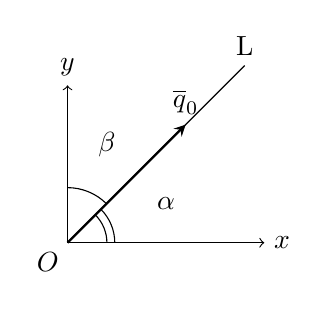
\begin{tikzpicture}[scale=0.5]
	\draw[->] (0,0) -- (5,0) node[right] {$x$};
	\draw[->] (0,0) -- (0,4) node[above] {$y$};
		
	\draw (0,0) -- (4.5,4.5) node[above] {L};			
	\draw[-stealth, thick] (0,0) -- (3,3) node[above] {$\overline{q}_0$};
	\draw (-0.5,-0.5) node{$O$};
	
	\draw[black] (1,0) arc (0:45:1);
	\draw[black] (1.2,0) arc (0:45:1.2);
	\draw (2.5,1) node{$\alpha$};
	
	\draw[black] (0,1.4) arc (90:45:1.4);
	\draw (1,2.5) node{$\beta$};
\end{tikzpicture}}
\parbox{\textwidth - 3.6cm}{
	Розглянемо довільну пряму $L \nparallel Ox$. Нехай $\alpha$ --- це кут нахилу $L$
	до осі $Ox$ (якщо $L \parallel Ox$, то $\alpha = 0$), $\beta$ --- це кут між прямою $L$
	та віссю $Oy$, $\overline{q}(l,m)$ --- це напрямний вектор прямої $L$, $\overline{q}_0$ ---
	це його орт-вектор. Тоді $\overline{q}_0 = (\cos \alpha, \cos \beta) = (\cos \alpha, \sin \alpha)$ (при
	цьому враховано, що $\alpha + \beta = \dfrac{\pi}{2}$). 
}

У цьому випадку канонічне рівняння прямої L буде мати вигляд:

$$\dfrac{x - x_0}{\cos\alpha} = \dfrac{y - y_0}{\sin\alpha}$$

Звідси $y - y_0 = \tg\alpha(x - x_0)$. Якщо позначити $k = \tg\alpha$ --- кутовий коефіцієнт,
то отримаємо рівняння прямої з кутовим коефіцієнтом:
$y - y_0 = k(x - x_0),$
що проходить через точку $M_0(x_0, y_0)$.
Останнє рівняння можна переписати у вигляді:

$$y = kx + b,$$

де $b = y_0 - kx_0$ --- величина відрізка, який відсікає $L$ на осі $Oy$. 

\section{Кут між двома прямими}

Кут між двома прямими дорівнює меншому з кутів між їх нормальними або
напрямними векторами. Розглянемо три випадки.

1. Прямі задано загальними рівняннями:

$$\begin{array}{l}
	L_1: A_1x + B_1y + C_1 = 0, \overline{n}_1(A_1,B_1); \\
	L_2: A_2x + B_2y + C_2 = 0, \overline{n}_2(A_2,B_2); \\
\end{array}$$

$$\cos(\widehat{L_1,L_2})
= \cos(\widehat{\overline{n}_1, \overline{n}_2})
= \dfrac{|A_1A_2 + B_1B_2|}{\sqrt{A_1^2+ B_1^2}\sqrt{A_2^2+ B_2^2}}.$$

2. Прямі задано у канонічному вигляді:

$$\begin{array}{l}
	L_1: \dfrac{x - x_1}{l_1} = \dfrac{y - y_1}{m_1}, \overline{q}_1(l_1,m_1); \\
	L_2: \dfrac{x - x_2}{l_2} = \dfrac{y - y_2}{m_2}, \overline{q}_2(l_2,m_2); \\
\end{array}$$

$$\cos(\widehat{L_1,L_2})
= \cos(\widehat{\overline{q}_1, \overline{q}_2})
= \dfrac{|l_1l_2 + m_1m_2|}{\sqrt{l_1^2+ m_1^2}\sqrt{l_2^2+ m_2^2}}.$$

3. Прямі задано рівняннями з кутовими коефіцієнтами: 

$$\begin{array}{l}
	L_1: y = k_1x + b_1, k_1 = \tg\alpha_1; \\
	L_2: y = k_2x + b_2, k_2 = \tg\alpha_2; \\
\end{array}$$

$$\tg(\widehat{L_1,L_2})
= \tg(\alpha_2 - \alpha_1)
= \left|\dfrac{\tg\alpha_2 - \tg\alpha_1}{1+\tg\alpha_1\tg\alpha_2}\right|
= \dfrac{k_2 - k_1}{1+k_1k_2}.$$

\newpage

\parbox{\textwidth - 0.6cm}{\section{Умови перпендикулярності і паралельності прямих}}

Паралельність або перпендикулярність двох прямих рівнозначна
паралельності або перпендикулярності нормальних або напрямних векторів. Тому
відповідно до вигляду рівнянь, якими задані прямі (див. пункти 1 – 3 попереднього
розділу), маємо:

\subsection*{Умови паралельності $L_1 \parallel L_2$:}

\begin{enumerate}
	\item $\overline{n}_1 \parallel \overline{n}_2$ або $\frac{A_1}{A_2} = \frac{B_1}{B_2}$;
	\item $\overline{q}_1 \parallel \overline{q}_2$ або $\frac{l_1}{l_2} = \frac{m_1}{m_2}$;
	\item $k_1 = k_2$.
\end{enumerate}

\subsection*{Умови перпендикулярності $L_1 \perp L_2$:}

\begin{enumerate}
	\item $\overline{n}_1 \perp \overline{n}_2$ або $A_1A_2 + B_1B_2 = 0$;
	\item $\overline{q}_1 \perp \overline{q}_2$ або $l_1l_2 + m_1m_2 = 0$;
	\item $k_1k_2 = -1$.
\end{enumerate}

\section{Нормальне рівняння прямої}

Нехай $L$ --- пряма, що не проходить через початок координат. Проведемо
нормальний вектор $\overline{n}$ так:
\begin{enumerate}
	\item його початок --- в точці $(0,0)$, а кінець лежить на прямій;
	\item $|\overline{n}| = p>0$ (такий вектор єдиний!).
	\item Кут $\alpha$ --- це кут між віссю $OX$ і $\overline{n}$, який відраховується проти годинникової стрілки.
\end{enumerate}

Нехай точка $M(x,y) \in L$. Тоді $\overline{OM}(x,y)$ --- це її радіус-вектор, $\overline{n}_0$ --- це ортвектор
нормального вектора $\overline{n}$: $\overline{n}_0 = (\cos\alpha,\cos\beta) = (\cos\alpha,\sin\alpha)$. При
цьому враховано, що $\alpha + \beta = \dfrac{\pi}{2}$.

\noindent\parbox{3.7cm}{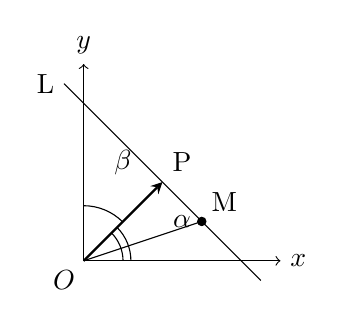
\begin{tikzpicture}[scale=0.5]
	\draw[->] (0,0) -- (5,0) node[right] {$x$};
	\draw[->] (0,0) -- (0,5) node[above] {$y$};
	\draw (-0.5,-0.5) node{$O$};			
			
	\draw (4.5,-0.5) -- (-0.5,4.5) node[left] {L};			
	\draw[-stealth, thick] (0,0) -- (2,2) node[above right] {P};
			
	\draw[black] (1,0) arc (0:45:1);
	\draw[black] (1.2,0) arc (0:45:1.2);
	\draw (2.5,1) node{$\alpha$};
	
	\draw[black] (0,1.4) arc (90:45:1.4);
	\draw (1,2.5) node{$\beta$};
			
	\draw (0,0) -- (3,1) node[above right] {M};
	\filldraw[black] (3,1) circle (3pt);
\end{tikzpicture}}
\parbox{\textwidth - 3.8cm}{
	Мають місце наступні співвідношення:

	$p = |OP|
	= \text{пр}_{\overline{n}}\overline{OM} = \text{пр}_{\overline{n}_0}\overline{OM}
	= |OM|\cos(\widehat{\overline{n}_0,OM})
	= |OM|\dfrac{(\overline{n}_0,\overline{OM})}{|\overline{n}_0||\overline{OM}|}
	= \dfrac{(\overline{n}_0,\overline{OM})}{|\overline{n}_0|}
	= x\cos\alpha + y\sin\alpha$.
	
	Отримали рівняння
	$x\cos\alpha + y\sin\alpha = 0$,	
	--- це \textbf{нормальне рівняння прямої $L$}, де $p$ --- це відстань від початку
	координат до прямої $L$.
}

\parbox{\textwidth - 0.6cm}{\section{Зведення загального рівняння прямої до нормального вигляду}}

Розглянемо загальне рівняння прямої $L: Ax + By + C= 0$, та нормальне
рівняння цієї прямої: $x\cos\alpha + y\sin\alpha - p = 0$.

Для того, щоб рівняння були рівносильними, достатньо, щоб їх коефіцієнти
були пропорційними: $\dfrac{\cos\alpha}{A} = \dfrac{\sin\alpha}{b} = \dfrac{-p}{C} = \mu$, де $\mu$ --- це
\textbf{нормуючий множник}. Тоді $\cos\alpha = \mu A, \sin\alpha = \mu B, -p = \mu C$. Звідси визначимо $\mu$:

$$\mu^2(A^2 + B^2) = \cos^2\alpha + \sin^2\alpha = 1 \Rightarrow \mu = \dfrac{1}{\pm\sqrt{A^2 + B^2}}.$$

Знак $\mu$ визначається рівністю $\mu C = -p$. Оскільки $p \geq 0$, то знак нормуючого
множника $\mu$ є протилежним до знаку $C$. Отже, \textbf{нормальне рівняння прямої} $L$ буде
мати вигляд

$\mu(Ax+By+C) = 0$, де $\mu = \dfrac{-\text{sign} C}{\sqrt{A^2 + B^2}}$ --- нормуючий множник.

\begin{example}
	Звести рівняння прямої $L : 3x-4y+25 = 0$ до нормального виду.
\end{example}
\begin{solution}
	Знайдемо нормуючий множник:

	$\mu = -\dfrac{1}{\sqrt{3^2 + (-4)^2}}$.
	Тоді $-\frac{3}{5} x + \frac{4}{5} y - 5 = 0$ --- нормальне рівняння $L$, де
	$\cos\alpha = -\frac{3}{5}, \sin\alpha = \frac{4}{5}, p = 5$ --- довжина перпендикуляра,
	опущеного з точки O на цю пряму. 
\end{solution}

\section{Відхилення і відстань від точки до прямої}

\parbox{4.5cm}{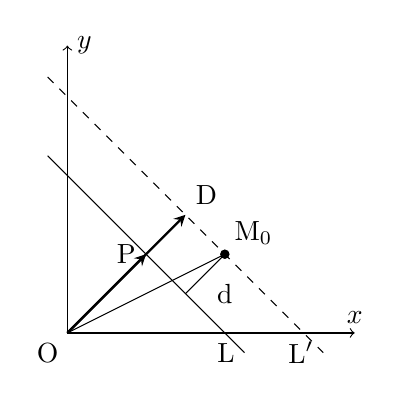
\begin{tikzpicture}[scale=0.5]
	\draw[->] (0,0) -- (7.3,0) node[above] {$x$};
	\draw[->] (0,0) -- (0,7.3) node[right] {$y$};
	\draw (-0.5,-0.5) node{O};
	%\draw[gray, dashed] (0,0) grid (7.3,7.3);
				
	\draw (-0.5,4.5) -- (4.5,-0.5) node[left] {L};
	\draw[dashed] (-0.5,6.5) -- (6.5,-0.5) node[left] {L$'$};
	\draw[-stealth, thick] (0,0) -- (2,2) node[left] {P};
	\draw[-stealth, thick] (0,0) -- (3,3) node[above right] {D};
		
	\draw (0,0) -- (4,2) node[above right] {M$_0$};
	\draw (3,1) -- (4,2);
	\draw (4,1) node{d};
	\filldraw[black] (4,2) circle (3pt);
\end{tikzpicture}}
\parbox{\textwidth - 4.6cm}{
	Нехай задано пряму $L$ , точку $M_0(x_0,y_0)\not\in L$,
	відстань від якої до даної прямої дорівнює
	$d = \rho(M_0, L) > 0$. Точка $O(0,0)$ --- це
	початок координат.

	Нехай пряма $L$ задається нормальним
	рівнянням: $x\cos\alpha + y\sin\alpha - p = 0$.
}

\begin{definition}
	\textbf{Відхилення} точки $M_0$ від прямої $L$ --- це число

	$$\delta_{M_0,L}\left\{\begin{array}{l}
		d\text{, якщо точки } M_0 \text{ і } O \text{ лежать по різні сторони прямої;} \\
		-d\text{, якщо точки } M_0 \text{ і } O \text{ лежать по один бік від прямої.} \\
	\end{array}\right.$$
\end{definition}


Обчислимо відхилення $\delta_{M_0,L}$. Для цього через точку $M_0$ проведемо пряму $L'$,
паралельну $L$. Побудуємо $OD \perp L'$. Тоді рівняння $L'$ має вигляд:

$$x\cos\alpha + y\sin\alpha - p - \delta_{M_0,L} = 0.$$

Але координати точки $M_0(x_0,y_0)$ задовольняють це рівняння, тому
$x_0\cos\alpha + y_0\sin\alpha - p - \delta_{M_0,L} = 0$.

Таким чином, відхилення точки $M_0$ від прямої $L$ обчислюється за формулою:
$$\delta_{M_0,L} = x_0\cos\alpha + y_0\sin\alpha - p$$

(для того, щоб знайти відхилення точки $M_0$ від прямої $L$ , потрібно підставити
координати цієї точки в нормальне рівняння даної прямої).

Відстань від точки $M_0(x_0,y_0) \not\in L$ до прямої $L$ обчислюється таким чином:
$$d = |\delta_{M_0,L}| = |x_0\cos\alpha + y_0\sin\alpha - p|$$.

Якщо ж пряма задається загальним рівнянням, то 
$$d = \dfrac{|Ax_0 + By_0 + C|}{\sqrt{A^2 + B^2}}$$.

\begin{problem}
	З’ясувати, в якому куті (гострому чи тупому), утвореному при перетині
	прямих $L_1$ та $L_2$, знаходиться точка $M_0(-2,2)$, якщо $L_1: 2x - y + 2 = 0$, 
	$L_2: 4x + y - 4 = 0$. В яких кутах (суміжних чи вертикальних) знаходяться точка
	$M_0$ та початок координат $O(0,0)$? 
\end{problem}
\begin{solution}
	З’ясуємо, який кут (гострий чи тупий) утворюють орти
	нормальних векторів прямих $L_1$ та $L_2$. Спочатку запишемо рівняння даних прямих
	у нормальному вигляді:
	
	$$\begin{array}{ll}
		L_1: -\dfrac{1}{\sqrt{5}}(2x - y + 2) = 0; & \overline{n}_1^0 = -\dfrac{1}{\sqrt{5}}(2,-1) = \dfrac{1}{\sqrt{5}}(-2,1);  \\
		L_1: \dfrac{1}{\sqrt{17}}(4x + y - 4) = 0; & \overline{n}_2^0 = \dfrac{1}{\sqrt{17}}(4,1);  \\
	\end{array}$$
	
	\noindent\parbox{4.5cm}{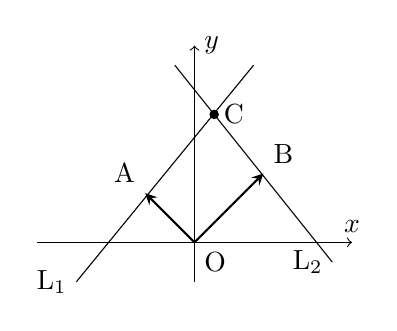
\begin{tikzpicture}[scale=0.5]
		\draw[->] (-4,0) -- (4,0) node[above] {$x$};
		\draw[->] (0,-1) -- (0,5) node[right] {$y$};
		\draw (0,0) node[below right]{O};
			
		\draw (1.5,4.5) -- (-3,-1) node[left] {L$_1$};
		\draw (-0.5,4.5) -- (3.5,-0.5) node[left] {L$_2$};
		\draw[-stealth, thick] (0,0) -- (-1.25,1.25) node[above left] {A};
		\draw[-stealth, thick] (0,0) -- (1.75,1.75) node[above right] {B};
		\filldraw (0.5,3.25) circle (3pt) node[right]{C};
	\end{tikzpicture}}
	\parbox{\textwidth - 4.6cm}{
		Оскільки скалярний добуток

		$$(\overline{n}_1^0,\overline{n}_2^0) = \frac{1}{\sqrt{5}\sqrt{17}}(-8+1) < 0,$$
		
		то кут $AOB$
		між векторами $\overline{n}_1^0$ та $\overline{n}_2^0$ --- тупий. У
		чотирикутнику $AOBC$ $\angle A$ та $\angle B$ --- прямі,
		$\angle AOB$ --- тупий, тому $\angle ACB$ --- гострий.
		
		Отже, початок координат $O(0,0)$ знаходиться в гострому куті, утвореному при
		перетині прямих $L_1$ та $L_2$.
	}
	
	Знайдемо відхилення точки $M_0(-2,2)$ від даних прямих.
	
	\noindent\parbox{2.4cm}{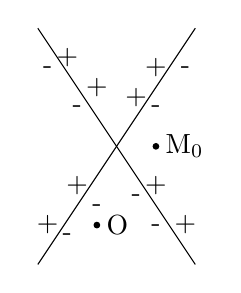
\begin{tikzpicture}[scale=0.5]
		\draw (-2,3) -- (2,-3);
		\draw (-2,-3) -- (2,3);
				
		\draw (1,1) node{-};
		\draw (1.75,2) node{-};
		\draw (0.5,1.25) node{+};
		\draw (1,2) node{+};
				
		\draw (-0.5,1.5) node{+};
		\draw (-1.25,2.25) node{+};
		\draw (-1,1) node{-};
		\draw (-1.75,2) node{-};
				
		\draw (1,-1) node{+};
		\draw (1.75,-2) node{+};
		\draw (0.5,-1.25) node{-};
		\draw (1,-2) node{-};
				
		\draw (-0.5,-1.5) node{-};
		\draw (-1.25,-2.25) node{-};
		\draw (-1,-1) node{+};
		\draw (-1.75,-2) node{+};
				
		\filldraw (1,0) circle (2pt) node[right]{M$_0$};
		\filldraw (-0.5,-2) circle (2pt) node[right]{O};
	\end{tikzpicture}}
	\parbox{\textwidth - 2.5cm}{
		$\delta_{M_0,L_1} = -\dfrac{1}{\sqrt{5}}(-4 -2 +2) = \dfrac{4}{\sqrt{5}} > 0;$
	
		$\delta_{M_0,L_2} = \dfrac{1}{\sqrt{17}}(-8 +2 -4) = -\dfrac{10}{\sqrt{17}} < 0;$
	
		Дві прямі, що перетинаються, ділять площину на
		чотири області. На рисунку зображено знаки відхилень
		точок, які лежать в кожній з чотирьох областей, при умові, що початок координат
		$O(0,0)$ знаходиться в гострому куті.
	}
	
	Враховуючи знаки відхилень точки $M_0$ від даних прямих, робимо висновок,
	що точка $M_0$ лежить в тупому куті, утвореному при перетині прямих $L_1$ та $L_2$.
	
	Точки $O(0,0)$ та $M_0$ лежать в суміжних кутах. 
\end{solution}

\section{Рівняння пучка (низки) прямих}

\begin{definition}
	\textbf{Пучок прямих (низка прямих)} на площині з центром у даній точці --- це  
	сукупність прямих, що проходить через цю точку.
\end{definition}

Якщо задана точка $M_0(x_0,y_0)$, то рівняння $A(x - x_0) + B(y - y_0) = 0$ при
змінних коефіцієнтах $A$ і $B$, а також рівняння $y-y_0 = k(x-x_0)$ при змінному $k$
є рівняннями пучка (низки) прямих з центром у точці $M_0$.

Пучок прямих можна задати довільними двома прямими, які перетинаються у
точці $M_0$:

$$\begin{array}{l}
	L_1: A_1x + B_1y + C_1 = 0,\\
	L_2: A_2x + B_2y + C_2 = 0.\\
\end{array}$$

Рівняння пучка прямих із центром у точці $M_0$ можна записати, не визначаючи
координат $M_0$:

$$A_1x + B_1y + C_1 + \lambda(A_2x + B_2y + C_2) = 0.$$

Щоб із пучка прямих виділити певну пряму, потрібно задати додаткову умову
для знаходження параметра $\lambda$, що відповідає шуканій прямій. 

